% Options for packages loaded elsewhere
\PassOptionsToPackage{unicode}{hyperref}
\PassOptionsToPackage{hyphens}{url}
%
\documentclass[
]{article}
\usepackage{lmodern}
\usepackage{amsmath}
\usepackage{ifxetex,ifluatex}
\ifnum 0\ifxetex 1\fi\ifluatex 1\fi=0 % if pdftex
  \usepackage[T1]{fontenc}
  \usepackage[utf8]{inputenc}
  \usepackage{textcomp} % provide euro and other symbols
  \usepackage{amssymb}
\else % if luatex or xetex
  \usepackage{unicode-math}
  \defaultfontfeatures{Scale=MatchLowercase}
  \defaultfontfeatures[\rmfamily]{Ligatures=TeX,Scale=1}
\fi
% Use upquote if available, for straight quotes in verbatim environments
\IfFileExists{upquote.sty}{\usepackage{upquote}}{}
\IfFileExists{microtype.sty}{% use microtype if available
  \usepackage[]{microtype}
  \UseMicrotypeSet[protrusion]{basicmath} % disable protrusion for tt fonts
}{}
\makeatletter
\@ifundefined{KOMAClassName}{% if non-KOMA class
  \IfFileExists{parskip.sty}{%
    \usepackage{parskip}
  }{% else
    \setlength{\parindent}{0pt}
    \setlength{\parskip}{6pt plus 2pt minus 1pt}}
}{% if KOMA class
  \KOMAoptions{parskip=half}}
\makeatother
\usepackage{xcolor}
\IfFileExists{xurl.sty}{\usepackage{xurl}}{} % add URL line breaks if available
\IfFileExists{bookmark.sty}{\usepackage{bookmark}}{\usepackage{hyperref}}
\hypersetup{
  hidelinks,
  pdfcreator={LaTeX via pandoc}}
\urlstyle{same} % disable monospaced font for URLs
\usepackage[margin=1in]{geometry}
\usepackage{graphicx}
\makeatletter
\def\maxwidth{\ifdim\Gin@nat@width>\linewidth\linewidth\else\Gin@nat@width\fi}
\def\maxheight{\ifdim\Gin@nat@height>\textheight\textheight\else\Gin@nat@height\fi}
\makeatother
% Scale images if necessary, so that they will not overflow the page
% margins by default, and it is still possible to overwrite the defaults
% using explicit options in \includegraphics[width, height, ...]{}
\setkeys{Gin}{width=\maxwidth,height=\maxheight,keepaspectratio}
% Set default figure placement to htbp
\makeatletter
\def\fps@figure{htbp}
\makeatother
\setlength{\emergencystretch}{3em} % prevent overfull lines
\providecommand{\tightlist}{%
  \setlength{\itemsep}{0pt}\setlength{\parskip}{0pt}}
\setcounter{secnumdepth}{5}
\usepackage{booktabs}
\usepackage{longtable}
\usepackage{array}
\usepackage{multirow}
\usepackage{wrapfig}
\usepackage{float}
\usepackage{colortbl}
\usepackage{pdflscape}
\usepackage{tabu}
\usepackage{threeparttable}
\usepackage{threeparttablex}
\usepackage[normalem]{ulem}
\usepackage{makecell}
\usepackage{xcolor}
\ifluatex
  \usepackage{selnolig}  % disable illegal ligatures
\fi

\author{}
\date{\vspace{-2.5em}}

\begin{document}

\begin{minipage}{2cm}
    
\includegraphics[width=1.2\textwidth]{archivos-rmd/logo-uc.jpg}
\end{minipage}

\begin{flushleft}
\noindent \textsc{Pontificia Universidad Cat\'olica de Chile \\
LET0010 - Habilidades Comunicativas para Estadísticos} \\
\noindent Segundo Semestre del 2020
\end{flushleft}

\vspace{10mm}
\begin{center}
\textbf{ \Large{Identificación de variables influyentes en el rendimiento escolar de estudiantes secundarios}}
\end{center}

\begin{flushright}
\noindent \textbf{Profesora}: Riva Quiroga\\
\noindent \textbf{Nombre}: Eduardo Vásquez
\end{flushright}

\vspace{10mm}

\renewcommand{\tablename}{Tabla}

\hypertarget{resumen}{%
\section{Resumen}\label{resumen}}

La Organización de las Naciones Unidas (ONU) presentó en el año 2015 un
plan de acción para el desarrollo sostenible, compuesto por 17
objetivos, entre los cuales se encuentra el garantizar una educación
inclusiva, equitativa y de calidad, para todos. Dado que estos objetivos
no están progresando a la velocidad necesaria para ser completados a
tiempo, se busca a través de este informe identificar las variables
estadísticamente significantes que influyen en el rendimiento escolar de
los estudiantes, para así a futuro poder buscar soluciones que se
enfoquen en estas, acelerando la mejoría de la educación entregada. Así,
en primer lugar, se da una vista general de los datos utilizados,
correspondientes a atributos de estudiantes pertenecientes a dos
escuelas en Portugal, separados por las asignaturas de matemáticas y
portugués. En segundo lugar, se realiza un análisis exploratorio de los
datos, en particular de la variable de interés: las notas finales.
Luego, se identifican las variables estadísticamente significativas para
cada una de las asignaturas, con las que después se ajustan los modelos
de regresión lineal respectivos. Además, se realiza un análisis de
supuestos del modelo y se entrega una transformación de los datos para
que los supuestos sí se cumplan. Finalmente, se presentan cuales son las
variables influyentes buscadas. Además, se formulan hipótesis sobre por
qué lo son, así como posibles soluciones a implementar. Se da cuenta
también de las limitaciones del modelo de regresión, así como aspectos a
considerar en futuros informes, como el uso de datos nacionales y
regionales.

\hypertarget{introducciuxf3n}{%
\section{Introducción}\label{introducciuxf3n}}

Durante septiembre del año 2015, los 193 estados miembros de la
Organización de las Naciones Unidas (ONU) decidieron, a través de la
Asamblea General, elaborar un plan de acción para el desarrollo
sostenible, conocida como la Agenda 2030 {[}1{]}. Este plan de acción
constituye ``un llamamiento universal a la acción para poner fin a la
pobreza, proteger el planeta y mejorar las vidas y las perspectivas de
las personas en todo el mundo'' {[}2{]}. Está compuesto por 17
objetivos, que se traducen en 169 metas más específicas que pueden ser
medidas de manera objetiva. Entre estos objetivos se encuentran, por
ejemplo, el fin de la pobreza, hambre cero, igualdad de género y acción
por el clima.

Uno de los problemas más importantes que se han encontrado a partir de
estos objetivos es que no están progresando a la velocidad o tasa
requerida, por lo que está en duda su posible completitud para el 2030
{[}2{]}. Dentro de estas metas se encuentra una de vital importancia
para todos, y sobre todo para los niños y jóvenes, quienes serán los
adultos del mañana: garantizar una educación inclusiva, equitativa y de
calidad, además de promover oportunidades de aprendizaje durante toda la
vida para todos. Sobre este objetivo, en el último reporte del año 2019,
se presenta que aún hay 617 millones de niños y adolescentes que no
alcanzan el nivel mínimo de competencia en lectura y matemáticas, y que
750 millones de adultos aún son analfabetos, de los cuales dos tercios
corresponden a mujeres {[}3, p.~7{]}. La importancia de este objetivo es
grande, debido a que la educación es fundamental para la movilidad
socioeconómica ascendente y la salida de la pobreza {[}4{]}. Además, una
educación de baja calidad provoca que muchos de los estudiantes no
posean las herramientas y aptitudes necesarias para hacer frente a una
economía mundial altamente compleja {[}3{]}, por lo que este objetivo
está muy correlacionado con los demás y, por lo tanto, su logro es
deseable.

Dado el problema anterior es que se desea poder identificar los factores
más influyentes en el rendimiento escolar de los estudiantes, para así
tomar medidas concretas e inmediatas que se enfoquen en estos, lo que
permitiría alcanzar el cuarto objetivo para el año 2030. Para lograr
esto, en el presente informe se analizará una base de datos disponible
en \emph{Kaggle} {[}5{]} sobre las notas obtenidas en dos asignaturas,
matemáticas y portugués, por diferentes estudiantes en dos colegios de
Portugal, la cual incluye atributos como el sexo, la edad, información
demográfica e información familiar. Así, para identificar lo señalado,
se realizarán diferentes análisis estadísticos, con lo que se obtienen
los atributos que son significativos en poder predecir el rendimiento
académico de los alumnos.

El informe se organiza en cuatro secciones: en primer lugar, se
presentan los diferentes atributos disponibles en la base de datos y se
describe el contexto en que estos se obtuvieron. Luego, se realiza un
análisis exploratorio inicial de los datos, principalmente a través de
gráficos, lo que permitirá identificar de manera preliminar atributos
significativos en el problema. En tercer lugar, se identifican las
variables significativas, se ajusta un modelo de regresión lineal
múltiple con estas variables y se muestran los resultados en formato de
tablas. Además se estudiará si el modelo es correcto a través de pruebas
de diagnósticos sobre los supuestos de éste, junto a posibles
transformaciones. Finalmente, se entrega una conclusión junto a
recomendaciones acerca de posibles medidas a tomar para algunos de los
atributos considerados significativos, así como futuras oportunidades de
estudio y los problemas de alcance del modelo presentado.

\hypertarget{metodologuxeda}{%
\section{Metodología}\label{metodologuxeda}}

\hypertarget{datos}{%
\subsection{Datos}\label{datos}}

Las bases de datos que usaremos en este informe fueron obtenidas a
partir de encuestas realizadas en dos escuelas de Portugal, Gabriel
Pereira y Mousinho da Silveira, a diferentes estudiantes que cursaban
alguna de las asignaturas de matemáticas o portugués. Es así como
obtenemos dos bases diferentes, una para cada asignatura.

Estas bases de datos poseen un número distinto de estudiantes en cada
una. En el caso de matemáticas tenemos un total de 395 observaciones,
mientras que en portugués tenemos un total de 649.

Para cada una de estas observaciones existen un total de 29 variables
registradas, entre las cuales se encuentra nuestra variable de interés:
la nota final. Estas variables fueron traducidas del inglés a partir de
la base original y, además, se les colocó un nombre más comprensible.
Podemos ver en la siguiente tabla los nombres de los atributos presentes
en la base de datos final a utilizar, en conjunto con su tipo y una
breve descripción de cada uno:

\begin{longtabu} to \linewidth {>{}l>{}l>{\raggedright\arraybackslash}p{30em}}
\caption{\label{tab:tabla variables}Atributos registrados de los estudiantes}\\
\toprule
Variable & Tipo & Descripcion\\
\midrule
\endfirsthead
\caption[]{Atributos registrados de los estudiantes \textit{(continuación)}}\\
\toprule
Variable & Tipo & Descripcion\\
\midrule
\endhead

\endfoot
\bottomrule
\endlastfoot
\textcolor{red}{\textbf{\cellcolor{gray!6}{escuela}}} & \cellcolor{gray!6}{categórica} & \cellcolor{gray!6}{Escuela del estudiante. 'GP': Gabriel Pereira, 'MS': Mousinho da Silveira}\\
\textcolor{red}{\textbf{sexo}} & categórica & Sexo del estudiante\\
\textcolor{red}{\textbf{\cellcolor{gray!6}{edad}}} & \cellcolor{gray!6}{numérica} & \cellcolor{gray!6}{Edad del estudiante}\\
\textcolor{red}{\textbf{tipo\_hogar}} & categórica & Tipo de hogar del estudiante (Urbano o Rural)\\
\textcolor{red}{\textbf{\cellcolor{gray!6}{tamano\_familia}}} & \cellcolor{gray!6}{categórica} & \cellcolor{gray!6}{Tamaño de la familia. Indica si el tamaño es igual o menor a 3,  o mayor que 3}\\
\addlinespace
\textcolor{red}{\textbf{estado\_padres}} & categórica & Estado de convivencia de los padres\\
\textcolor{red}{\textbf{\cellcolor{gray!6}{educacion\_madre}}} & \cellcolor{gray!6}{numérica} & \cellcolor{gray!6}{Nivel educacional de la madre}\\
\textcolor{red}{\textbf{educacion\_padre}} & numérica & Nivel educacional del padre\\
\textcolor{red}{\textbf{\cellcolor{gray!6}{trabajo\_madre}}} & \cellcolor{gray!6}{categórica} & \cellcolor{gray!6}{Tipo de trabajo de la madre}\\
\textcolor{red}{\textbf{trabajo\_padre}} & categórica & Tipo de trabajo del padre\\
\addlinespace
\textcolor{red}{\textbf{\cellcolor{gray!6}{apoderado}}} & \cellcolor{gray!6}{categórica} & \cellcolor{gray!6}{Apoderado del estudiante}\\
\textcolor{red}{\textbf{tiempo\_viaje}} & numérica & Tiempo de viaje del hogar a la escuela del estudiante\\
\textcolor{red}{\textbf{\cellcolor{gray!6}{tiempo\_estudio}}} & \cellcolor{gray!6}{numérica} & \cellcolor{gray!6}{Tiempo de estudio semanal del estudiante}\\
\textcolor{red}{\textbf{reprobaciones}} & numérica & Número de reprobaciones en asignaturas pasadas\\
\textcolor{red}{\textbf{\cellcolor{gray!6}{soporte\_educacional}}} & \cellcolor{gray!6}{categórica} & \cellcolor{gray!6}{Indica si el estudiante recibe soporte educacional extra de la escuela}\\
\addlinespace
\textcolor{red}{\textbf{soporte\_familiar}} & categórica & Indica si el estudiante recibe soporte educacional de su familia\\
\textcolor{red}{\textbf{\cellcolor{gray!6}{pago\_extra}}} & \cellcolor{gray!6}{categórica} & \cellcolor{gray!6}{Indica si el estudiante recibe clases extras pagadas}\\
\textcolor{red}{\textbf{actividades}} & categórica & Indica si el estudiante participa de actividades extracurriculares\\
\textcolor{red}{\textbf{\cellcolor{gray!6}{ed\_superior}}} & \cellcolor{gray!6}{categórica} & \cellcolor{gray!6}{Indica si el estudiante desea ingresar a la educación superior}\\
\textcolor{red}{\textbf{internet}} & categórica & Indica si el estudiante posee acceso a internet desde su hogar\\
\addlinespace
\textcolor{red}{\textbf{\cellcolor{gray!6}{relacion\_amorosa}}} & \cellcolor{gray!6}{categórica} & \cellcolor{gray!6}{Indica si el estudiante está en una relación romántica}\\
\textcolor{red}{\textbf{relacion\_familiar}} & numérica & Indica la calidad de la relación familiar en una escala del 1 al 5\\
\textcolor{red}{\textbf{\cellcolor{gray!6}{tiempo\_libre}}} & \cellcolor{gray!6}{numérica} & \cellcolor{gray!6}{Indica la cantidad de tiempo libre del estudiante a través de una escala del 1 al 5}\\
\textcolor{red}{\textbf{salir}} & numérica & Indica cuánto tiempo sale el estudiante con sus amigos a través de una escala del 1 al 5\\
\textcolor{red}{\textbf{\cellcolor{gray!6}{alcohol\_dia}}} & \cellcolor{gray!6}{numérica} & \cellcolor{gray!6}{Indica la cantidad de consumo de alcohol en días de semana a través de una escala del 1 al 5}\\
\addlinespace
\textcolor{red}{\textbf{alcohol\_fin\_de\_semana}} & numérica & Indica la cantidad de consumo de alcohol durante los fines de semana a través de una escala del 1 al 5\\
\textcolor{red}{\textbf{\cellcolor{gray!6}{salud}}} & \cellcolor{gray!6}{numérica} & \cellcolor{gray!6}{Indica el estado de salud actual del estudiante a través de una escala del 1 al 5}\\
\textcolor{red}{\textbf{ausencias}} & numérica & Indica la cantidad de faltas a la escuela del estudiante\\
\textcolor{red}{\textbf{\cellcolor{gray!6}{nota\_final}}} & \cellcolor{gray!6}{numérica} & \cellcolor{gray!6}{Calificación final del estudiante a través de una escala del 0 al 20}\\*
\end{longtabu}

Podemos notar desde ya un problema con nuestros datos, el cual es la
posible subjetividad de estos. Por ejemplo, si tomamos la variable
salud, no sabemos realmente si lo que contestó el estudiante en la
encuesta refleja verdaderamente su estado de salud. Vemos entonces que
todas las variables con escala del 1 al 5 pueden ser consideradas
subjetivas y, por lo tanto, debemos tener esto en consideración al
momento de presentar resultados.

No solo la subjetividad es un problema en estas variables, sino que
además el alumno puede responder lo que él desee en la encuesta, por
razones como que el estudiante no se sienta cómodo al dar a conocer su
situación. Por ejemplo, podría esconder su verdadera cantidad de consumo
de alcohol durante la semana, o podría mentir sobre la calidad de su
relación familiar.

También es importante considerar los tipos de datos que se indican en la
tabla, como por ejemplo el nivel educacional, indicada como numérica.
Esto es ya que en la base de datos se presentan los diferentes niveles
educacionales a través de números, pero, ya que estos están de manera
ascendente, no deberíamos tener problemas en el análisis posterior.

Por último, las variables comprendidas entre
\textbf{soporte\_educacional} e \textbf{internet}, ambas incluidas, son
respondidas solamente con un sí o un no.

\hypertarget{anuxe1lisis-exploratorio}{%
\subsection{Análisis Exploratorio}\label{anuxe1lisis-exploratorio}}

Antes de pasar a nuestro análisis de regresión podemos tratar de
explorar nuestros datos de manera gráfica, para así poder entenderlos de
mejor manera, o incluso poder obtener resultados o atisbos del
comportamiento de estos desde un principio.

En primer lugar, es importante analizar lo que queremos predecir o
entender, lo cual en nuestro caso son las notas finales. Las notas
finales en Portugal están dadas como números enteros desde el 0 hasta el
20, donde una calificación igual o mayor a 10 es considerada suficiente
y, por lo tanto, una nota menor es reprobatoria {[}6{]}. Para analizar
entonces las notas finales, vemos los siguientes gráficos de barras, uno
para matemáticas y uno para portugués, que indican la proporción con que
cada una de las notas se encuentra en nuestra base de datos:

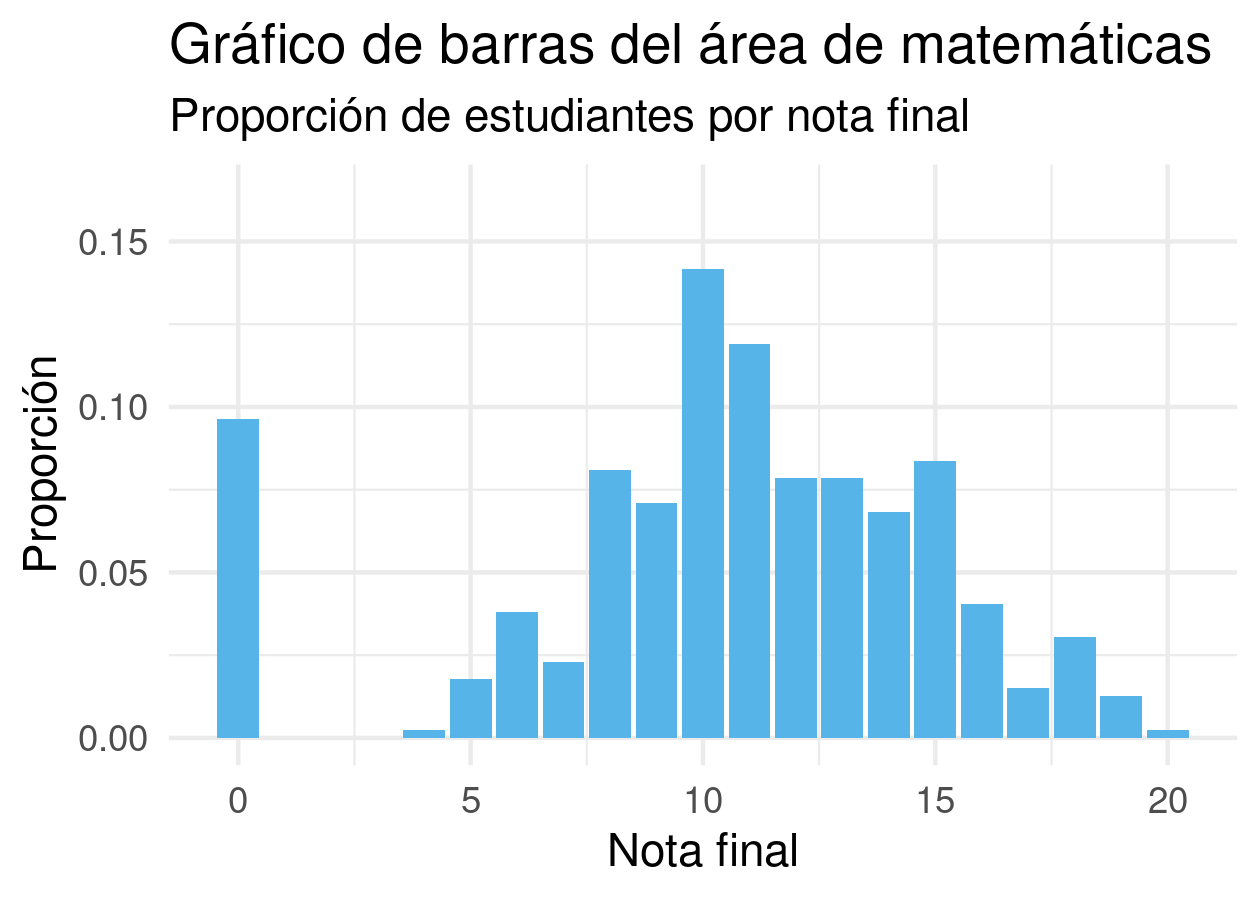
\includegraphics[width=0.5\linewidth]{/mnt/Data/Estadística UC/LET0010 - Habilidades Comunicativas para Estadísticos/proyecto-let0010/figuras/01_notas-mat}
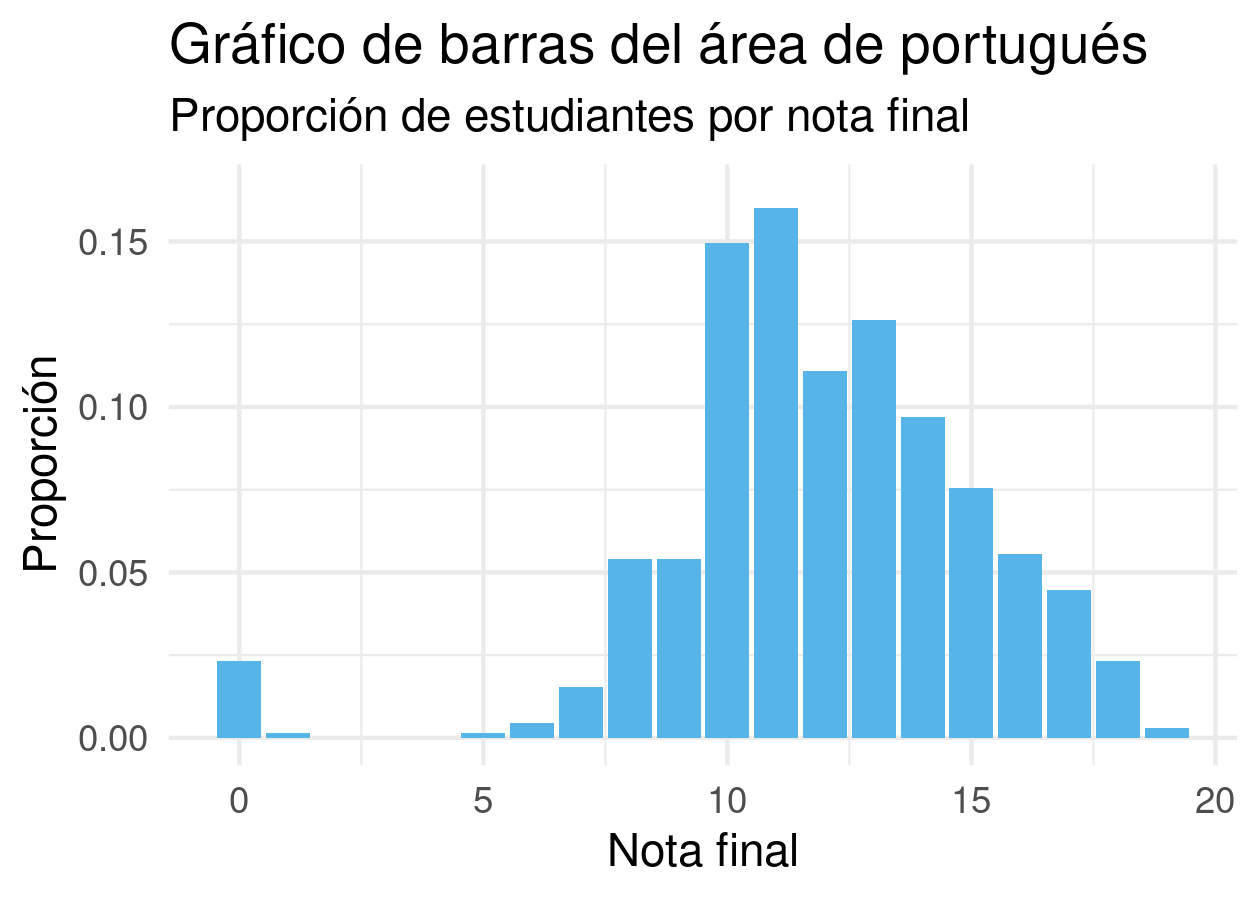
\includegraphics[width=0.5\linewidth]{/mnt/Data/Estadística UC/LET0010 - Habilidades Comunicativas para Estadísticos/proyecto-let0010/figuras/02_notas-por}

Notamos a partir de estas gráficas tres características importantes: en
primer lugar, la proporción de alumnos con la menor nota posible (0) en
matemáticas es mayor que la proporción de alumnos con la menor nota
posible en portugués, correspondiente a cerca de un 10\% de los alumnos
en matemáticas y a aproximadamente un 2.5\% de los alumnos en portugués,
como lo indica la altura de la barra en 0. En segundo lugar, la
distribución de las notas en matemáticas pareciera ser más simétrica que
la distribución de notas en portugués, dado que las calificaciones de
portugués parecen concentrarse mayoritariamente a la derecha de 10, en
vez de concentrarse uniformemente hacia ambos lados. Así, vemos que la
proporción de alumnos que aprueba portugués es mayor que la proporción
de alumnos que aprueba matemáticas. Finalmente, notamos que la
proporción de alumnos con notas entre 1 y 5 es casi cero para ambas
asignaturas.

En cuanto a la segunda característica mencionada en el párrafo anterior,
podemos hacer el cálculo exacto, a partir de lo cual obtenemos que un
32.9\% de los estudiantes en el curso de matemáticas reprobaron,
mientras que en el caso de la asignatura de portugués reprobó solamente
un 15.4\%.

Además de obtener información gráfica sobre nuestra variable respuesta,
también podemos calcular algunos estadísticos de resumen como la media,
la mediana y cuartiles, los cuales se presentan en la siguiente tabla:

\begin{longtable}[t]{lrrrrrr}
\caption{\label{tab:tabla estadisticos promedio}Estadísticas de resumen de las notas finales}\\
\toprule
Asignatura & Mínimo & Primer cuartil & Media & Mediana & Tercer cuartil & Máximo\\
\midrule
\cellcolor{gray!6}{Matemáticas} & \cellcolor{gray!6}{0} & \cellcolor{gray!6}{8} & \cellcolor{gray!6}{10.41519} & \cellcolor{gray!6}{11} & \cellcolor{gray!6}{14} & \cellcolor{gray!6}{20}\\
Portugués & 0 & 10 & 11.90601 & 12 & 14 & 19\\
\bottomrule
\end{longtable}

A partir de lo anterior podemos observar que, por ejemplo, en la
asignatura de matemáticas el 50\% de los estudiantes tiene una nota
final menor o igual a 11, mientras que en portugués este valor
corresponde a una nota final de 12.

Ahora que ya tenemos una idea de cómo se comporta nuestra variable de
interés, es entonces válido preguntarnos cómo se comporta esta misma
variable al hacer divisiones en la base de datos a partir de los otros
atributos, denominados atributos explicativos. Como primera variable
explicativa a utilizar para desagregar nuestra información usaremos
\textbf{escuela}, lo cual nos puede servir para descubrir si es que
acaso existe una diferencia de rendimiento entre ambos colegios y, en
caso de que así sea, estudiar más en profundidad las razones de esto.
Para esto vemos la siguiente figura, que muestra un diagrama de cajas
separado por escuela para cada una de las asignaturas:

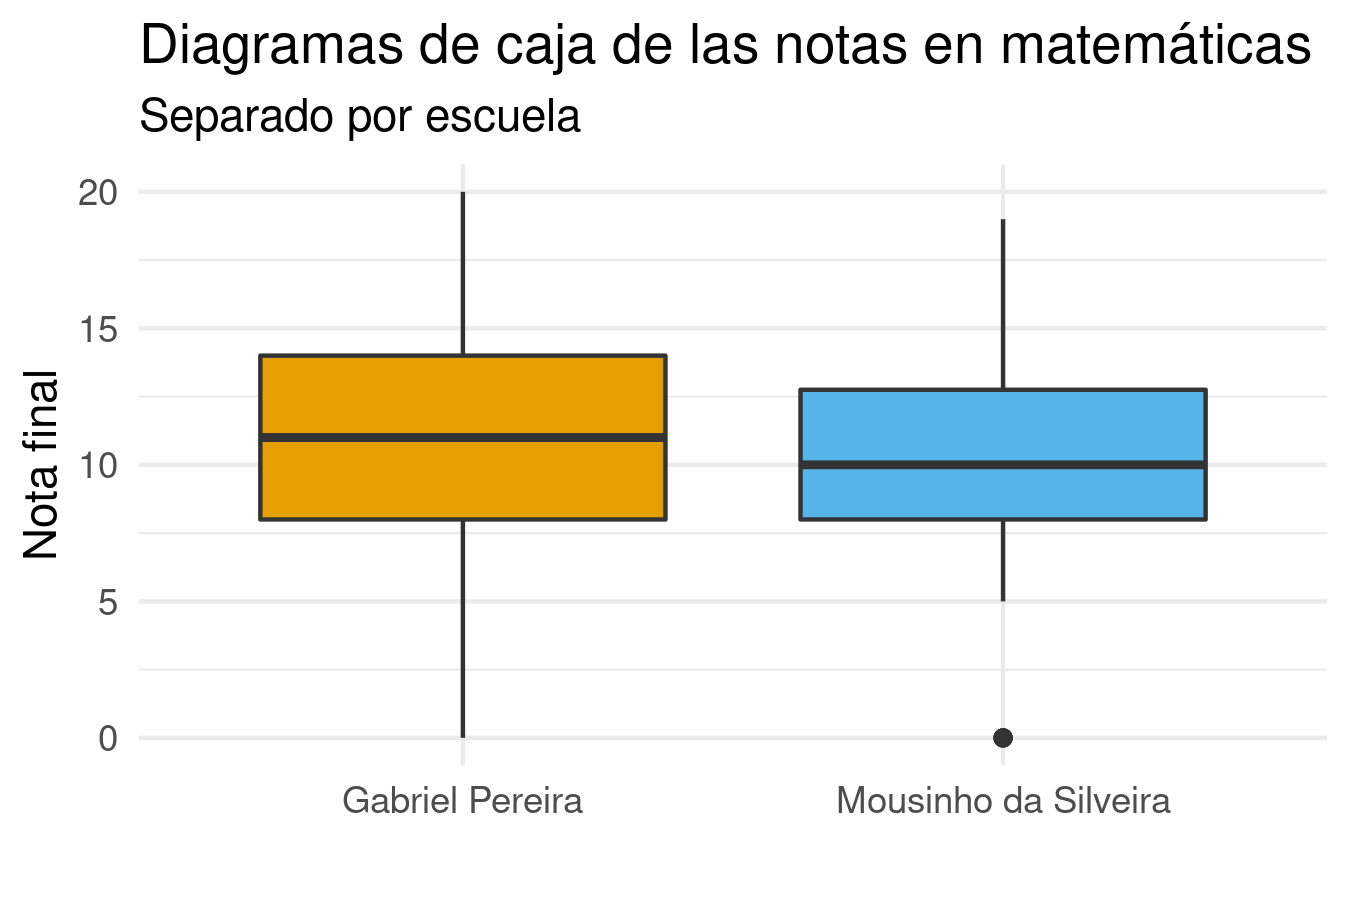
\includegraphics[width=0.5\linewidth]{/mnt/Data/Estadística UC/LET0010 - Habilidades Comunicativas para Estadísticos/proyecto-let0010/figuras/05_diferencia-notas-mat-escuela}
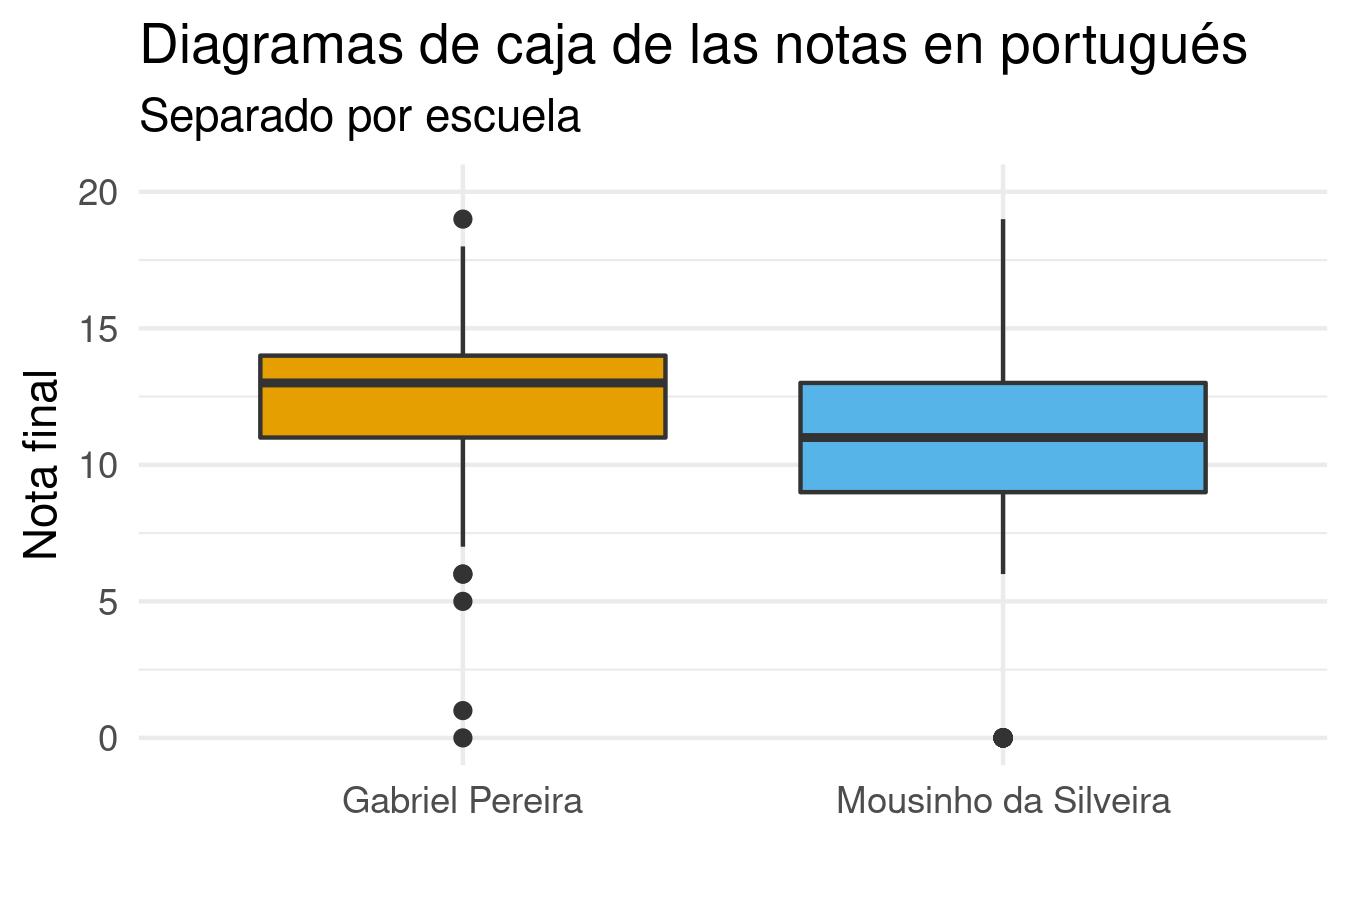
\includegraphics[width=0.5\linewidth]{/mnt/Data/Estadística UC/LET0010 - Habilidades Comunicativas para Estadísticos/proyecto-let0010/figuras/06_diferencia-notas-por-escuela}

En los gráficos anteriores es posible observar que, en cuanto a las
notas de matemáticas, la mediana de estas en la escuela Gabriel Pereira,
representada por la línea horizontal que cruza la caja, es mayor que la
de la escuela Mousinho da Silveira, aunque con una diferencia no tan
considerable. En cambio, en el gráfico de la derecha notamos una clara
diferencia de medianas entre ambas escuelas, donde la mediana en la
escuela Gabriel Pereira es considerablemente mayor que en la escuela
Mousinho da Silveira. Notamos además que los cuatro diagramas de caja
incluyen al cero y, por lo tanto, el problema de alumnos que reprueban
con nota cero se da en ambas escuelas y en ambas asignaturas.

Como una segunda variable explicativa a usar para estudiar nuestra
variable respuesta podemos utilizar el atributo \textbf{sexo}. Descubrir
si hay diferencias de notas en cuanto al sexo del estudiante es de vital
importancia en el objetivo de la ONU, ya que se busca entregar una
educación inclusiva y equitativa. Nuevamente, presentamos una figura que
contiene los diagramas de caja respectivos, separados en este caso por
el atributo sexo, para cada una de las asignaturas:

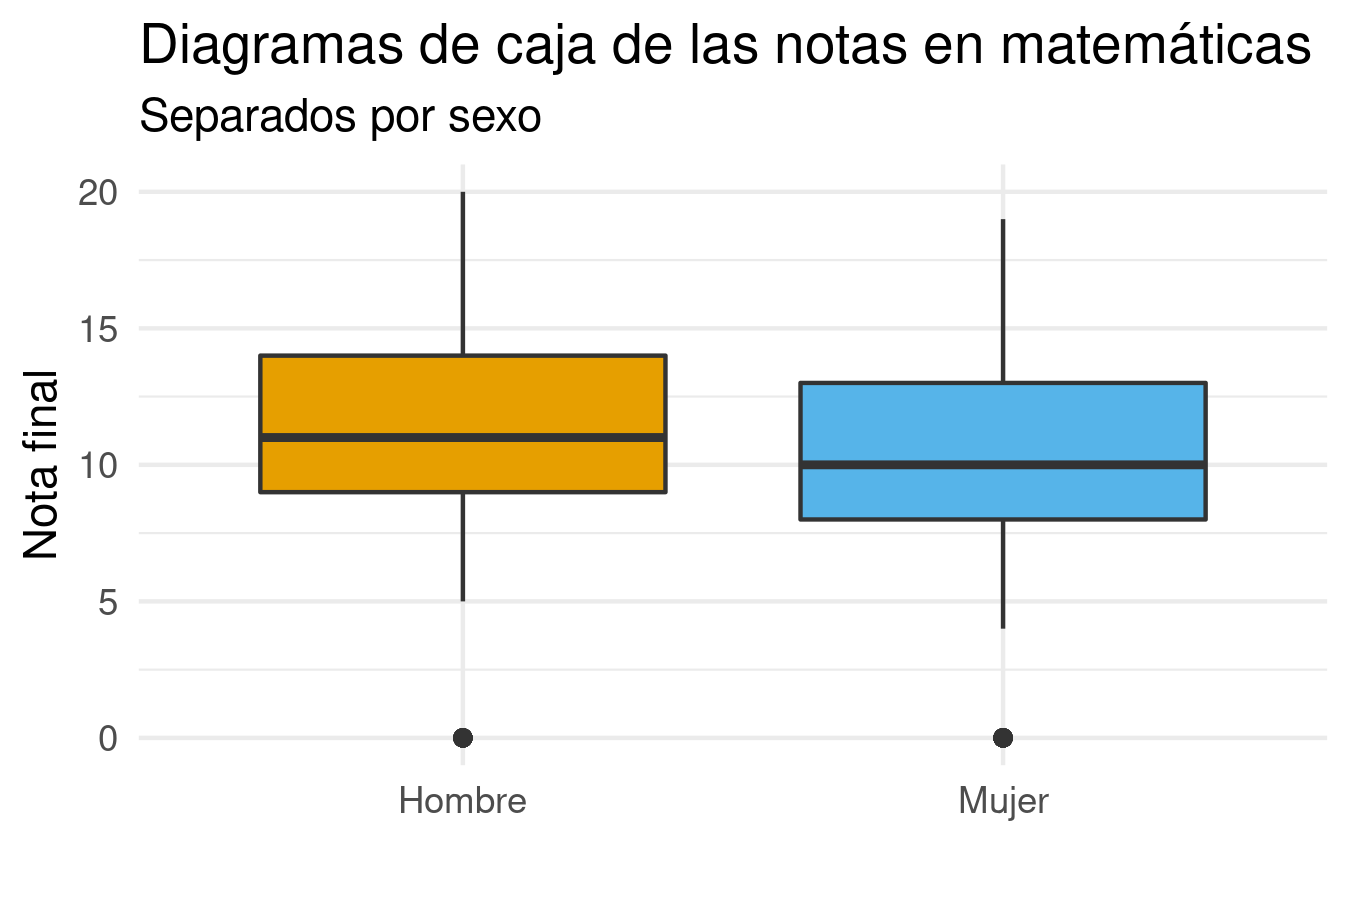
\includegraphics[width=0.5\linewidth]{/mnt/Data/Estadística UC/LET0010 - Habilidades Comunicativas para Estadísticos/proyecto-let0010/figuras/03_diferencia-notas-mat-sexo}
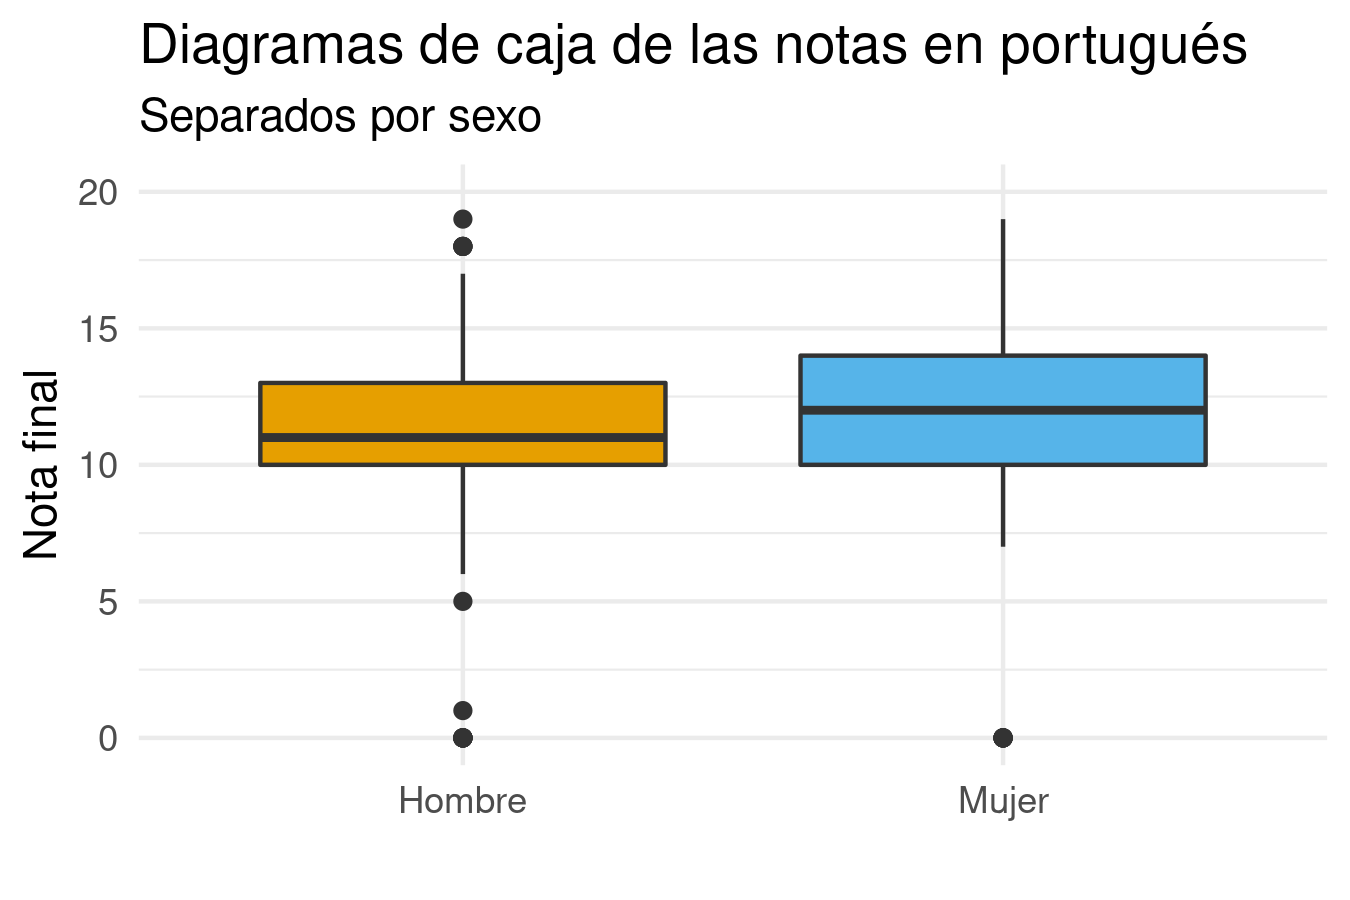
\includegraphics[width=0.5\linewidth]{/mnt/Data/Estadística UC/LET0010 - Habilidades Comunicativas para Estadísticos/proyecto-let0010/figuras/04_diferencia-notas-por-sexo}

Es posible notar en este caso que en cuanto a matemáticas, la mediana de
las notas obtenidas por los hombres, representada por la línea
horizontal que cruza la caja, es mayor, aunque por un margen bastante
pequeño, mientras que en el caso de portugués, son las mujeres quienes
poseen una mediana mayor.

De todas maneras, debemos tener cuidado con el análisis anterior, ya que
al estudiar gráficamente nuestra variable respuesta al desagregar por
una variable puede entregarnos resultados diferentes, e incluso
posiblemente contradictorios, que al momento de utilizar el conjunto
entero de variables explicativas. Por esto, pasamos a un análisis
estadístico más formal: el análisis de regresión.

\hypertarget{anuxe1lisis-de-regresiuxf3n}{%
\subsection{Análisis de Regresión}\label{anuxe1lisis-de-regresiuxf3n}}

Dado que nuestra variable respuesta es numérica, se realizará un
análisis de regresión para lograr identificar las variables
significativamente influyentes en el rendimiento escolar.

En primer lugar, debido a la gran cantidad de atributos que poseen
nuestras bases de datos, usaremos métodos de selección de variables para
identificar las variables estadísticamente significantes en explicar las
notas finales. Para esto usaremos un test chi-cuadrado de agregación de
atributos significativos con un valor de significancia del
\(\alpha = 0.1\). Este valor puede parecer alto, pero nos interesan
todas las variables que puedan tener una influencia en las notas
finales, por muy mínima que la significancia de esta influencia sea.

Luego, ajustamos nuestros modelos para obtener las estimaciones de los
coeficientes, lo que nos permite realizar predicciones acerca de las
notas finales de los estudiantes, así como medir la magnitud del impacto
que tienen cada una de las variables identificadas como significativas.

Finalmente, analizaremos dos supuestos del modelo: la normalidad de los
errores y la homocedasticidad, esto es, la varianza constante de los
errores, a través del test de Kolmogorov-Smirnov y el test de
Breusch-Pagan, respectivamente. La razón de esto es que si aquellos
supuestos no se cumplen, nuestros test de hipótesis utilizados para
elegir variables serán inexactos. En el caso de no cumplirse estas
suposiciones, buscaremos transformaciones de nuestra variable respuesta,
la nota final, a través de la transformación de Box-Cox, para luego
verificar nuevamente los supuestos al utilizar esta transformación.

\hypertarget{resultados}{%
\section{Resultados}\label{resultados}}

\hypertarget{notas-finales-en-matemuxe1ticas}{%
\subsection{Notas finales en
matemáticas}\label{notas-finales-en-matemuxe1ticas}}

\hypertarget{selecciuxf3n-de-variables-y-ajuste-del-modelo}{%
\subsubsection{Selección de variables y ajuste del
modelo}\label{selecciuxf3n-de-variables-y-ajuste-del-modelo}}

En cuanto a las notas finales de matemáticas podemos ver a través de la
siguiente tabla las variables seleccionadas por nuestro método y el
valor-p del test que utilizamos:

\begin{longtable}[t]{ll}
\caption{\label{tab:tabla variables mat}Atributos significativos en predecir la nota final en matemáticas}\\
\toprule
Variable & Valor-p\\
\midrule
\endfirsthead
\caption[]{Atributos significativos en predecir la nota final en matemáticas \textit{(continued)}}\\
\toprule
Variable & Valor-p\\
\midrule
\endhead

\endfoot
\bottomrule
\endlastfoot
\cellcolor{gray!6}{reprobaciones} & \cellcolor{gray!6}{0.00000}\\
educacion\_madre & 0.00365\\
\cellcolor{gray!6}{sexo} & \cellcolor{gray!6}{0.02002}\\
salir & 0.01748\\
\cellcolor{gray!6}{trabajo\_madre} & \cellcolor{gray!6}{0.02654}\\
\addlinespace
relacion\_amorosa & 0.04373\\
\cellcolor{gray!6}{soporte\_familiar} & \cellcolor{gray!6}{0.07858}\\
tiempo\_estudio & 0.07568\\
\cellcolor{gray!6}{ausencias} & \cellcolor{gray!6}{0.06817}\\*
\end{longtable}

Notamos que son 9 atributos en total considerados significativos, al
tener un valor-p menor a nuestro nivel de \(\alpha = 0.1\).

Luego, a partir de las variables elegidas por el método, ajustamos
nuestro modelo, de lo cual se obtienen las estimaciones de los
coeficientes, mostrados a través de la siguiente tabla:

\begin{longtable}[t]{lr}
\caption{\label{tab:tabla variables mat 2}Estimaciones de los coeficientes del modelo}\\
\toprule
Variable & Estimación\\
\midrule
\endfirsthead
\caption[]{Estimaciones de los coeficientes del modelo \textit{(continuación)}}\\
\toprule
Variable & Estimación\\
\midrule
\endhead

\endfoot
\bottomrule
\endlastfoot
\cellcolor{gray!6}{Intercepto} & \cellcolor{gray!6}{10.996}\\
reprobaciones & -1.965\\
\cellcolor{gray!6}{educacion\_madre} & \cellcolor{gray!6}{0.518}\\
salir & -0.488\\
\cellcolor{gray!6}{tiempo\_estudio} & \cellcolor{gray!6}{0.511}\\
ausencias & 0.048\\
\addlinespace[0.3em]
\multicolumn{2}{l}{\textbf{Sexo}}\\
\hspace{1em}\cellcolor{gray!6}{mujer} & \cellcolor{gray!6}{-1.228}\\
\addlinespace[0.3em]
\multicolumn{2}{l}{\textbf{Trabajo madre}}\\
\hspace{1em}otro & -0.095\\
\hspace{1em}\cellcolor{gray!6}{profesora} & \cellcolor{gray!6}{-0.431}\\
\hspace{1em}publico & 1.179\\
\hspace{1em}\cellcolor{gray!6}{salud} & \cellcolor{gray!6}{1.838}\\
\addlinespace[0.3em]
\multicolumn{2}{l}{\textbf{Relación amorosa}}\\
\hspace{1em}si & -1.042\\
\addlinespace[0.3em]
\multicolumn{2}{l}{\textbf{Soporte familiar}}\\
\hspace{1em}\cellcolor{gray!6}{si} & \cellcolor{gray!6}{-0.848}\\*
\end{longtable}

Estos resultados podemos interpretarlos de la siguiente manera: en
primer lugar vemos que la nota final esperada de los estudiantes en la
asignatura de matemáticas parte en 10.996, indicada por el intercepto.
Luego, tenemos que, por ejemplo, por cada vez que el o la estudiante
haya reprobado el curso anteriormente, esta nota final esperada
disminuye en un 1.965. Para las variables categóricas la interpretación
es la misma: si, por ejemplo, el estudiante se encuentra en una relación
amorosa, la nota esperada disminuye en un 1.04, o de la misma manera, si
la estudiante es mujer, la nota esperada disminuye en un 1.228.

\hypertarget{anuxe1lisis-de-supuestos}{%
\subsubsection{Análisis de supuestos}\label{anuxe1lisis-de-supuestos}}

Presentamos a través de la siguiente tabla los resultados del test de
Kolmogorov-Smirnov y del test de Breusch-Pagan:

\begin{longtable}[t]{lll}
\caption{\label{tab:resultados test mat}Resultados de los análisis de supuestos}\\
\toprule
Test & Valor del estadístico & Valor-p\\
\midrule
\cellcolor{gray!6}{Kolmogorov-Smirnov} & \cellcolor{gray!6}{0.073843} & \cellcolor{gray!6}{0.02693}\\
Breusch-Pagan & 19.381 & 0.07975\\
\bottomrule
\end{longtable}

A partir de estos resultados, y al usar un nivel de significancia del
\(\alpha = 0.05\), solamente podemos concluir la homocedasticidad de los
errores, debido a que el valor-p del test correspondiente de
Breusch-Pagan está por encima del nivel de significancia, pero no así en
el test de Kolmogorov-Smirnov. Por esta razón, debemos buscar alguna
transformación de la variable respuesta.

\hypertarget{transformaciuxf3n-de-la-variable-respuesta}{%
\subsubsection{Transformación de la variable
respuesta}\label{transformaciuxf3n-de-la-variable-respuesta}}

Debido a que en nuestro modelo ajustado no pudimos concluir la
normalidad de los errores, debemos buscar alguna transformación de
nuestra variable respuesta que nos permita concluir que los supuestos sí
se cumplen. Para esto usaremos la transformación de Box-Cox, la cual
toma nuestra variable respuesta \(Y\), correspondiente a la nota final,
y busca el valor de \(\lambda\) óptimo para:

\[
\frac{Y^\lambda - 1}{\lambda}
\]

tal que el valor del estadístico del test de Kolmogorov-Smirnov sea
mínimo (y podamos entonces concluir normalidad). Realizamos esta
búsqueda para diferentes valores de \(\lambda\) y se obtuvo un valor
óptimo de \(1.57\).

Finalmente, ajustamos nuestro modelo nuevamente, pero con nuestras notas
finales transformadas, y realizamos los tests de Kolmogorov-Smirnov y
Breusch-Pagan. Vemos los resultados de los tests en de la siguiente
tabla:

\begin{longtable}[t]{lll}
\caption{\label{tab:resultados test mat 2}Resultados de los análisis de supuestos con la variable respuesta transformada}\\
\toprule
Test & Valor del estadístico & Valor-p\\
\midrule
\cellcolor{gray!6}{Kolmogorov-Smirnov} & \cellcolor{gray!6}{0.02298} & \cellcolor{gray!6}{0.9852}\\
Breusch-Pagan & 19.976 & 0.06754\\
\bottomrule
\end{longtable}

A partir de estos resultados notamos ahora que, con un nivel de
significancia del \(\alpha = 0.05\), sí podemos concluir ambos supuestos
y, entonces, podemos concluir que nuestro método de selección de
variables es confiable para el caso de las notas finales en matemáticas.

\hypertarget{notas-finales-en-portuguuxe9s}{%
\subsection{Notas finales en
portugués}\label{notas-finales-en-portuguuxe9s}}

\hypertarget{selecciuxf3n-de-variables-y-ajuste-del-modelo-1}{%
\subsubsection{Selección de variables y ajuste del
modelo}\label{selecciuxf3n-de-variables-y-ajuste-del-modelo-1}}

En cuanto a las notas finales de portugués procedemos de la misma manera
que en el caso de las notas finales en matemáticas. Vemos a través de la
siguiente tabla las variables seleccionadas por nuestro método y el
valor-p del test que utilizamos:

\begin{longtable}[t]{ll}
\caption{\label{tab:tabla variables por}Atributos significativos en predecir la nota final en portugués}\\
\toprule
Variable & Valor-p\\
\midrule
\endfirsthead
\caption[]{Atributos significativos en predecir la nota final en portugués \textit{(continued)}}\\
\toprule
Variable & Valor-p\\
\midrule
\endhead

\endfoot
\bottomrule
\endlastfoot
\cellcolor{gray!6}{reprobaciones} & \cellcolor{gray!6}{0.000000}\\
escuela & 0.000000\\
\cellcolor{gray!6}{ed\_superior} & \cellcolor{gray!6}{0.000000}\\
tiempo\_estudio & 0.000036\\
\cellcolor{gray!6}{soporte\_educacional} & \cellcolor{gray!6}{0.000242}\\
\addlinespace
alcohol\_dia & 0.000192\\
\cellcolor{gray!6}{educacion\_madre} & \cellcolor{gray!6}{0.009292}\\
salud & 0.007633\\
\cellcolor{gray!6}{sexo} & \cellcolor{gray!6}{0.02617}\\
apoderado & 0.04177\\
\addlinespace
\cellcolor{gray!6}{relacion\_amorosa} & \cellcolor{gray!6}{0.07322}\\
edad & 0.0988\\*
\end{longtable}

Observamos en este caso que la cantidad de variables estadísticamente
significantes según nuestro método es mayor que los obtenidos en el
modelo de matemáticas, con un total de 12 atributos. Notamos también que
las variables consideradas significativas para portugués y matemáticas
son similares, pero no incluyen exactamente las mismas.

Luego, a partir de nuestras variables elegidas por el método, ajustamos
nuestro modelo, de lo cual se obtienen las estimaciones de los
coeficientes, mostrados a través de la siguiente tabla:

\begin{longtable}[t]{lr}
\caption{\label{tab:tabla variables por 2}Estimaciones de los coeficientes del modelo}\\
\toprule
Variable & Estimación\\
\midrule
\endfirsthead
\caption[]{Estimaciones de los coeficientes del modelo \textit{(continuación)}}\\
\toprule
Variable & Estimación\\
\midrule
\endhead

\endfoot
\bottomrule
\endlastfoot
\cellcolor{gray!6}{Intercepto} & \cellcolor{gray!6}{17.8509}\\
reprobaciones & -1.5026\\
\cellcolor{gray!6}{educacion\_madre} & \cellcolor{gray!6}{0.3032}\\
tiempo\_estudio & 0.4329\\
\cellcolor{gray!6}{alcohol\_dia} & \cellcolor{gray!6}{-0.3874}\\
salud & -0.1737\\
\cellcolor{gray!6}{edad} & \cellcolor{gray!6}{0.1566}\\
\addlinespace[0.3em]
\multicolumn{2}{l}{\textbf{Escuela}}\\
\hspace{1em}Mousinho da Silveira & -1.4312\\
\addlinespace[0.3em]
\multicolumn{2}{l}{\textbf{Educación superior}}\\
\hspace{1em}\cellcolor{gray!6}{si} & \cellcolor{gray!6}{1.8987}\\
\addlinespace[0.3em]
\multicolumn{2}{l}{\textbf{Soporte educacional}}\\
\hspace{1em}si & -1.3054\\
\addlinespace[0.3em]
\multicolumn{2}{l}{\textbf{Sexo}}\\
\hspace{1em}\cellcolor{gray!6}{mujer} & \cellcolor{gray!6}{0.5494}\\
\addlinespace[0.3em]
\multicolumn{2}{l}{\textbf{Apoderado}}\\
\hspace{1em}padre & 0.4667\\
\addlinespace[0.3em]
\multicolumn{2}{l}{\textbf{Relación amorosa}}\\
\hspace{1em}\cellcolor{gray!6}{si} & \cellcolor{gray!6}{-0.4387}\\*
\end{longtable}

Acá podemos interpretar los resultados de la misma manera que en el caso
de las notas finales en matemáticas. En primer lugar observamos que la
nota final esperada de los estudiantes en portugués parte en 17.8509.
Luego, tenemos que, por ejemplo, por cada unidad que aumenta el tiempo
de estudio del estudiante, su nota esperada aumenta en 0.4329, mientras
que por cada unidad que aumente su consumo de alcohol diario la nota
esperada disminuye en 0.3874. Para variables categóricas procedemos de
la misma manera, donde podemos ver que, por ejemplo, si el estudiante se
encuentra en la escuela Mousinho da Silveira, su nota esperada será
menor, al tener un valor estimado negativo, al igual que si el
estudiante recibe soporte educacional.

Notamos que en este caso obtenemos algunos resultados diferentes al caso
de matemáticas. Por ejemplo en portugués esperamos que la nota final
esperada aumente en 0.5494 si la estudiante es mujer, mientras que en
matemáticas la nota final esperada disminuye en 1.228. También tenemos
resultados similares, como que la nota final esperada en ambos casos es
menor si el o la estudiante se encuentra en una relación amorosa.

Finalmente, recordamos que en la sección de análisis exploratorio
descubrimos un hecho importante: la diferencia de notas entre escuelas
parecía ser significativa en la asignatura de portugués, pero no así en
matemáticas, visto a través de los diagramas de caja. En esta sección
confirmamos este hecho, al notar que la escuela fue considerada
significativa por nuestro método para el modelo de la asignatura de
portugués, mientras que en matemáticas no fue así.

\hypertarget{anuxe1lisis-de-supuestos-1}{%
\subsubsection{Análisis de supuestos}\label{anuxe1lisis-de-supuestos-1}}

Presentamos a través de la siguiente tabla los resultados del test de
Kolmogorov-Smirnov y del test de Breusch-Pagan:

\begin{longtable}[t]{lll}
\caption{\label{tab:resultados test por}Resultados de los análisis de supuestos}\\
\toprule
Test & Valor del estadístico & Valor-p\\
\midrule
\cellcolor{gray!6}{Kolmogorov-Smirnov} & \cellcolor{gray!6}{0.059992} & \cellcolor{gray!6}{0.018710}\\
Breusch-Pagan & 49.646 & 0.000002\\
\bottomrule
\end{longtable}

A partir de estos resultados, y al usar un nivel de significancia del
\(\alpha = 0.05\), no podemos concluir ninguno de los supuestos, ya que
en ninguno de los dos casos el valor-p se encuentra sobre este valor y,
por lo tanto, debemos buscar alguna transformación de la variable
respuesta

\hypertarget{transformaciuxf3n-de-la-variable-respuesta-1}{%
\subsubsection{Transformación de la variable
respuesta}\label{transformaciuxf3n-de-la-variable-respuesta-1}}

De manera similar al caso del modelo de matemáticas, debemos buscar
alguna transformación de las notas finales, dado que no podemos concluir
ninguno de los dos supuestos mencionados. Para esto usaremos nuevamente
el método transformación de Box-Cox, a partir del cual obtenemos un
valor de \(\lambda\) óptimo de \(1.34\).

Finalmente, ajustamos nuestro modelo nuevamente, pero con nuestras notas
finales transformadas, y realizamos los tests de Kolmogorov-Smirnov y
Breusch-Pagan. Vemos los resultados de los tests en la siguiente tabla:

\begin{longtable}[t]{lll}
\caption{\label{tab:resultados test por 2}Resultados de los análisis de supuestos con la variable respuesta transformada}\\
\toprule
Test & Valor del estadístico & Valor-p\\
\midrule
\cellcolor{gray!6}{Kolmogorov-Smirnov} & \cellcolor{gray!6}{0.040292} & \cellcolor{gray!6}{0.2427}\\
Breusch-Pagan & 45.001 & 0.00001\\
\bottomrule
\end{longtable}

Notamos ahora que, al tomar un nivel de significancia del
\(\alpha = 0.05\), sí podemos concluir la normalidad de los errores,
pero no fuimos capaces de arreglar el problema de no poder concluir el
supuesto de homocedasticidad.

\hypertarget{conclusiones}{%
\section{Conclusiones}\label{conclusiones}}

A través del desarrollo de este informe estudiamos, en primer lugar, las
características de nuestra variable de interés, que son las notas
finales. Observamos cómo estas distribuyen en cada asignatura, y
obtuvimos algunos estadísticos de interés. Las bajas notas finales de
los estudiantes nos entregan información sobre posibles problemas en la
educación, tanto de la parte que aprende como de la parte que enseña,
por lo que su estudio es importante para poder entregar una educación
inclusiva, equitativa y de calidad, tal como lo plantea el objetivo de
la ONU. En segundo lugar, nos enfocamos en encontrar las variables
significativas en poder predecir estas notas finales, separando entre
las asignaturas de portugués y matemáticas, debido a que ambas son
diferentes en sus métodos evaluativos y, posiblemente, de enseñanza, por
lo que no tendría sentido mezclar ambos análisis. Se logra así
identificar las variables significativas para cada asignatura, para
luego ajustar un modelo de regresión lineal múltiple en cada caso.
Finalmente, se estudió si es que estos modelos ajustados eran correctos
al analizar sus supuestos, en particular el supuesto de normalidad de
los errores y el de homocedasticidad. El incumplimiento de estos
supuestos provoca que nuestro método utilizado para obtener variables
significantes sea inexacto, por lo que es crucial que estos sí se
cumplan. Al realizar este análisis, llegamos a la conclusión de que para
el caso de matemáticas sí se cumplían ambas suposiciones, por lo que
nuestros resultados son confiables, pero en el caso de portugués no
podíamos deducir la homocedasticidad, por lo que debemos tener cuidado
con los resultados de este modelo.

Es así como a partir del análisis anterior podemos dar respuesta a
nuestro problema: identificar los factores más importantes que influyen
en el rendimiento escolar de los estudiantes. Tenemos entonces dos
respuestas, una para cada asignatura:

\begin{enumerate}
\def\labelenumi{\arabic{enumi}.}
\item
  Matemáticas: Dado que pudimos concluir que los errores distribuyen de
  manera normal y que la varianza de estos es constante, nuestro método
  utilizado para selección de variables es confiable y, entonces, las
  variables señaladas como significativas son las presentadas en la
  tabla 3. En cuanto al impacto que tiene cada una de estas variables en
  la nota final esperada del estudiante podemos observar la tabla 4.
  Dentro de esta última tabla podemos notar que el mayor coeficiente en
  valor absoluto es el correspondiente a \textbf{reprobaciones}, con un
  valor de -1.965, lo que nos dice que por cada vez que un estudiante
  reprueba anteriormente el curso, su nota final esperada disminuye en
  esa cantidad.
\item
  Portugués: En este caso no pudimos concluir que la varianza de los
  errores es constante, por lo que nuestro método no será exacto. De
  todas maneras, el supuesto más importante para el modelo de regresión
  utilizado es el de normalidad, por lo que los resultados presentes en
  la tabla 7 serán cercanos a los resultados reales. Deberíamos de todas
  maneras tener cuidado con estas variables, sobre todo con las más
  cercanas a \(0.1\), nuestro valor de significancia, que serían
  \textbf{edad} y \textbf{relacion\_amorosa}. En cuanto al impacto que
  tiene cada una de estas variables en la nota final esperada del
  estudiante podemos observar la tabla 8. Dentro de esta tabla podemos
  notar que el mayor coeficiente en valor absoluto es el correspondiente
  a \textbf{educacion\_superior}, con un valor de 1.8987, es decir, si
  el estudiante tiene en mente seguir estudiando, su nota final esperada
  es mayor.
\end{enumerate}

A partir de los resultados obtenidos podemos entonces generar hipótesis
acerca de las razones por las que algunas estas variables son
significativas en las notas finales:

\begin{enumerate}
\def\labelenumi{\arabic{enumi}.}
\item
  reprobaciones: Esta variable es considerada significativa en ambos
  casos y en ambas impactan de manera negativa la nota final esperada.
  Esto puede deberse a una mala reinserción de los estudiantes al
  momento de cursar la asignatura nuevamente, por lo que una posible
  solución es el acompañar a estos estudiantes a través de tutores que
  sean estudiantes que sí hayan aprobado el curso.
\item
  educacion\_madre: Esta variable es considerada significativa en ambos
  casos y en ambas impactan de manera positiva en la nota final
  esperada. Creemos entonces que existe una alta correlación entre la
  educación de los padres de los estudiantes con el rendimiento de
  estos, lo que puede deberse a un temprano acercamiento a la educación
  desde los padres hacia los hijos, así como una mayor valoración de la
  educación en la familia.
\item
  tiempo\_estudio: Esta variable es considerada significativa en ambos
  casos y en ambas impactan de manera positiva en la nota final
  esperada. Es importante entonces inculcarles a los estudiantes la
  importancia del estudio, pero también nos tenemos que hacer la
  siguiente pregunta: ¿hasta qué punto debiesen estudiar?, es decir, si
  los estudiantes deben dedicar todo su tiempo posible en estudiar, o si
  tienen el derecho de usar su tiempo libre como ellos quieran. Además,
  es importante estudiar el por qué algunos alumnos no logran dedicar
  más horas a su tiempo de estudio, ya que puede ser que no sea que no
  estudian porque no quieren, sino que mas bien porque no pueden.
\item
  sexo: Esta variable es considerada significativa en ambos casos, pero
  en la asignatura de matemáticas impacta de manera negativa el hecho de
  ser mujer, mientras que en portugués impacta de manera positiva. Es
  importante entonces el estudiar las razones por las que esto sucede,
  para luego buscar soluciones a este problema de desigualdad.
\item
  escuela: Esta variable es considerada significativa solamente en el
  caso de portugués, donde impacta de manera negativa si la escuela del
  estudiante es Mousinho da Silverira. Acá pueden haber muchas razones
  por las que esto ocurre, como puede ser que esta escuela entrega una
  educación de menor calidad, o también puede ser que es de mayor
  exigencia. Es entonces primordial descubrir la razón de este
  resultado, para así poder asegurar una educación equitativa para todos
  los estudiantes.
\end{enumerate}

El poder comprobar estas hipótesis, así como proponer nuevas, son el
próximo paso en poder avanzar en materia educacional para poder
completar a tiempo el objetivo educativo de la ONU. El poder esclarecer
las razones por la que las variables mencionadas son significantes en
predecir la nota final de la asignatura nos lleva a poder formular
soluciones pertinentes, que se deben implementar lo antes posible.
Lamentablemente esto se escapa del alcance de nuestro informe, ya que se
requieren conocimientos en materias de educación e implementación de
políticas educativas.

Finalmente, también se invita a realizar estudios que abarquen una
cantidad mayor de escuelas, ya que en este caso nuestra muestra
correspondía solamente a dos establecimientos, sin poder saber si es que
acaso estas son una buena representación de todas las escuelas en
Portugal. Se sugiere entonces realizar estas encuestas de manera
nacional o regional, lo que permitiría tener una mayor confianza en los
resultados obtenidos. Se invita también a realizar lo mismo pero en
diferentes países del mundo, ya que cada uno posee una realidad
distinta, por lo que también poseen problemas distintos y soluciones
distintas.

También, algo muy importante de notar, y que observamos en nuestro
análisis exploratorio, es que las notas finales encontradas en nuestras
bases de datos están representadas por números enteros, y no por números
continuos. Esto implica que el modelo utilizado de regresión lineal no
sería la mejor opción, por lo que debemos inclinarnos por modelos
lineales que trabajen con números enteros, como la regresión Poisson o
la regresión binomial, los cuales se escapan de nuestro alcance. Se deja
entonces abierta la posibilidad de repetir estos análisis a través de
metodologías que usen estos modelos más acordes a la situación del
problema.

\newpage

\hypertarget{referencias}{%
\section{Referencias}\label{referencias}}

{[}1{]} Asamblea General. Transformar nuestro mundo: la agenda 2030 para
el desarrollo sostenible. 2015. Disponible en:
\url{https://undocs.org/es/A/RES/70/1}

{[}2{]} Organización de las Naciones Unidas. La Agenda para el
Desarrollo Sostenible {[}Internet{]}. {[}fecha desconocida{]} {[}citado
el 2020 Dic 14{]}. Disponible en:
\url{https://www.un.org/sustainabledevelopment/development-agenda}.

{[}3{]} Organización de las Naciones Unidas. Informe de los objetivos de
desarrollo sostenible. 2019. Disponible en:
\url{https://unstats.un.org/sdgs/report/2019/The-Sustainable-Development-Goals-Report-2019_Spanish.pdf}.

{[}4{]} Organización de las Naciones Unidas. Objetivo 4: garantizar una
educación inclusiva, equitativa y de calidad y promover oportunidades de
aprendizaje durante toda la vida para todos {[}Internet{]}. {[}fecha
desconocida{]} {[}citado el 2020 Dic 14{]}. Disponible en:
\url{https://www.un.org/sustainabledevelopment/es/education/}

{[}5{]} Cortez P, Silva A. Using data mining to predict secondary school
student performance. EUROSIS. 2008.

{[}6{]} Diário da República Eletrónico. Decreto-Lei n.° 42/2005
{[}Internet{]}. 2005 {[}citado el 2020 Dic 14{]}. Disponible en:
\url{https://data.dre.pt/eli/dec-lei/42/2005/02/22/p/dre/pt/html}.

\end{document}
